\documentclass[11pt,a4paper]{article}
\usepackage[margin=1in]{geometry}
\usepackage[T1]{fontenc}
\usepackage[utf8]{inputenc}
\usepackage{lmodern}
\usepackage{setspace}
\usepackage{booktabs}
\usepackage{longtable}
\usepackage{array}
\usepackage{graphicx}
\usepackage{float}
\usepackage{hyperref}
\usepackage{enumitem}
\usepackage{amsmath}
\setlist{nosep}
\onehalfspacing

\title{Developer Guide --- Protein Enzyme Classification Project}
\author{}
\date{Last updated: March 2026}

\begin{document}
\maketitle

\tableofcontents
\newpage

\section{Project Overview}
This project implements a 7-class supervised classification system that predicts whether a
protein is an enzyme and, if so, its top-level Enzyme Commission (EC) class.

\begin{table}[H]
\centering
\caption{Class distribution used throughout training and evaluation.}
\begin{tabular}{lrrr}
\toprule
Class & Label & Count & Proportion \\
\midrule
0 & Not an enzyme & 32410 & 81.5\% \\
1 & Oxidoreductase & 1184 & 3.0\% \\
2 & Transferase & 2769 & 7.0\% \\
3 & Hydrolase & 2108 & 5.3\% \\
4 & Lyase & 600 & 1.5\% \\
5 & Isomerase & 411 & 1.0\% \\
6 & Ligase & 282 & 0.7\% \\
\bottomrule
\end{tabular}
\end{table}

Technology stack:
\begin{itemize}
\item Python 3.10+
\item scikit-learn, XGBoost, LightGBM, PyTorch
\item ESM-2 via fair-esm
\item BioPython for FASTA and ProtParam features
\item matplotlib, seaborn, SHAP
\end{itemize}

\section{Environment Setup}
\subsection{Prerequisites}
\begin{itemize}
\item Python $\ge$ 3.10
\item CUDA-capable GPU recommended for ESM extraction and fine-tuning
\item Approximately 12 GB disk for embeddings and checkpoints
\end{itemize}

\subsection{Installation}
\begin{verbatim}
# 1) Clone repository
git clone <repo-url>
cd protein-classification

# 2) Create venv
python -m venv .venv

# 3) Activate (Windows PowerShell)
.\.venv\Scripts\Activate.ps1

# 4) Install dependencies
pip install -r requirements.txt
\end{verbatim}

\section{Dataset Description}
Seven FASTA files in workspace root map to labels 0--6:
\begin{verbatim}
class0_rep_seq.fasta.txt
ec1_rep_seq.fasta.txt
ec2_rep_seq.fasta.txt
ec3_rep_seq.fasta.txt
ec4_rep_seq.fasta.txt
ec5_rep_seq.fasta.txt
ec6_rep_seq.fasta.txt
\end{verbatim}

All sequences are representative and non-homologous after clustering.
No additional deduplication is required.

\section{Architecture Overview}
\begin{figure}[H]
\centering
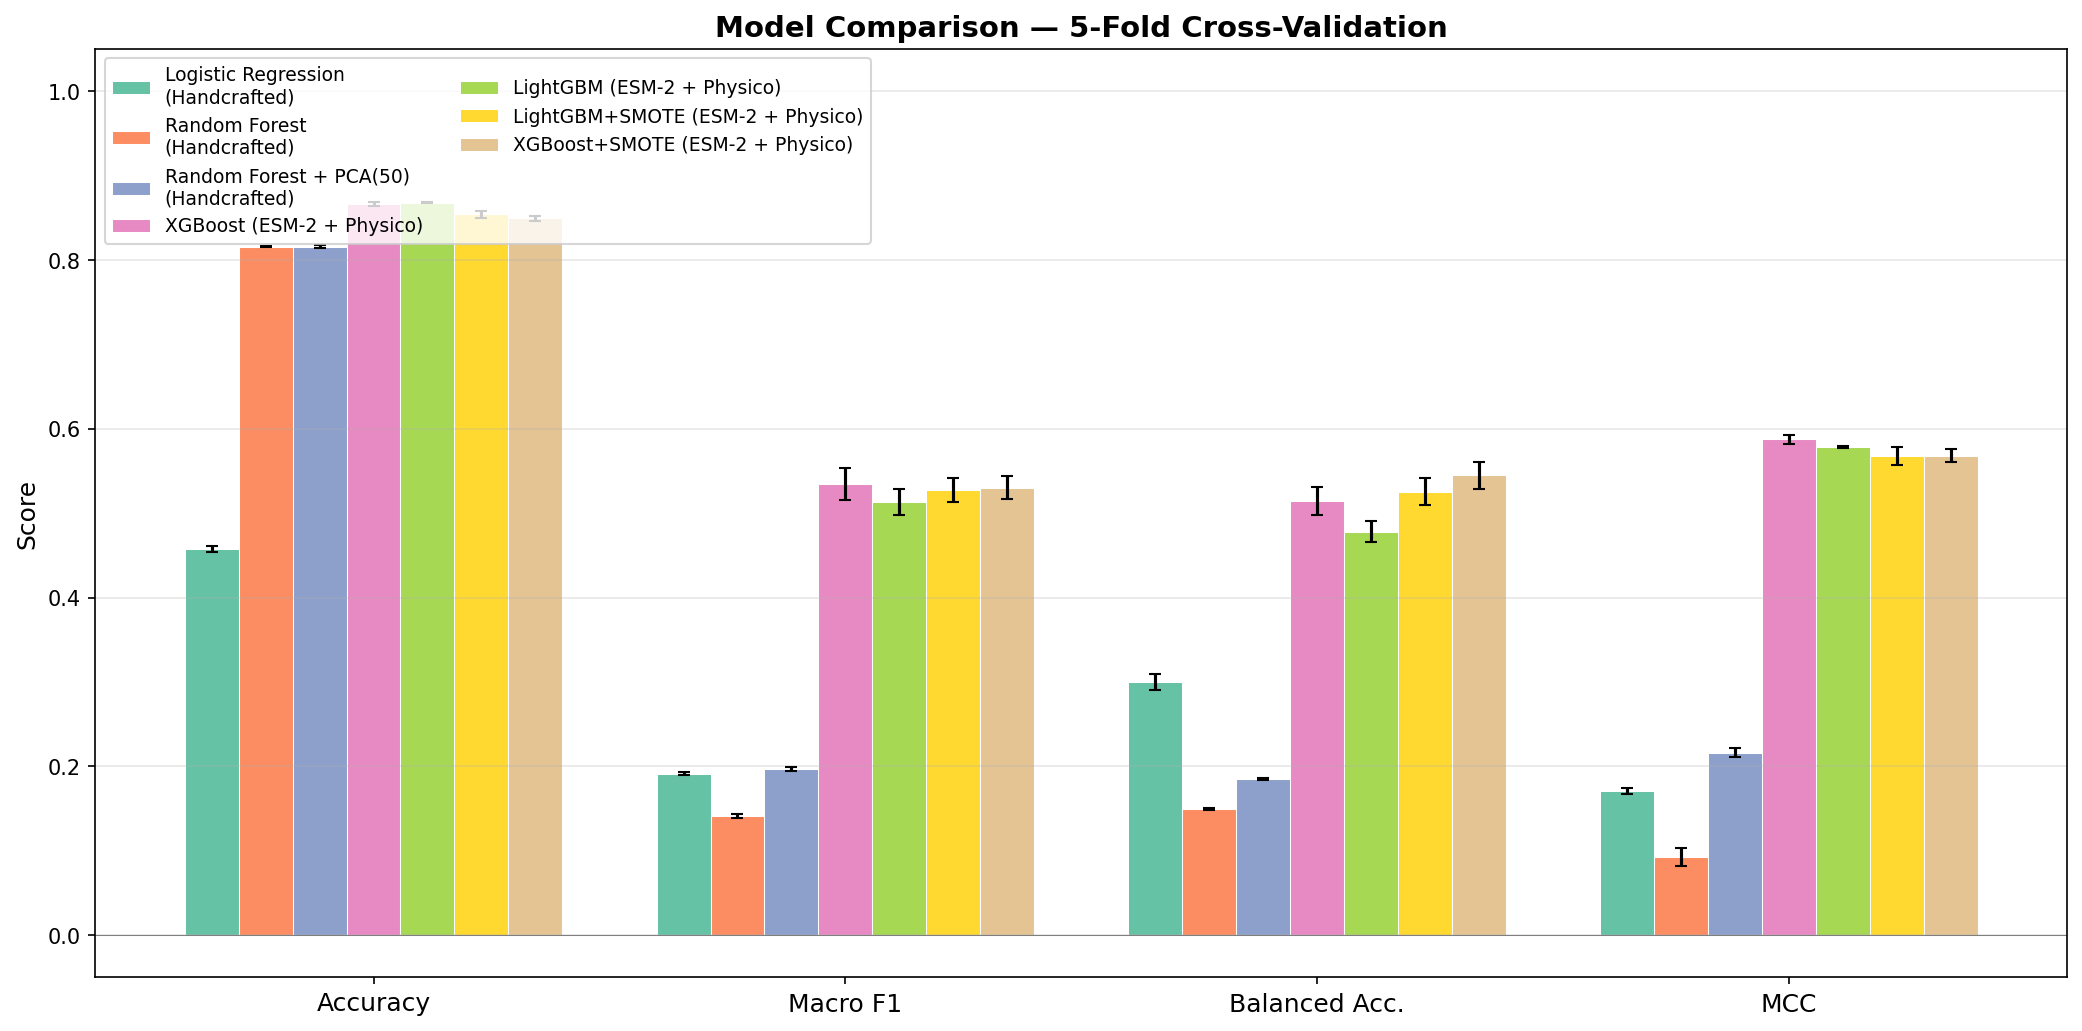
\includegraphics[width=0.92\textwidth]{../figures/model_comparison.png}
\caption{High-level model family outcomes used to guide architecture choices.}
\end{figure}

Data and module flow:
\begin{enumerate}
\item \texttt{src/data\_loading.py}: FASTA parsing and CV split generation
\item \texttt{src/features/*}: composition, physicochemical, ESM-2 embeddings
\item \texttt{src/training.py}: leak-safe CV and threshold optimisation utilities
\item \texttt{src/models/*}: baseline, advanced, finetune, ensemble
\item \texttt{src/evaluation.py}, \texttt{src/interpretability.py}, \texttt{src/confidence.py}
\item \texttt{src/predict\_blind.py}: FASTA to final formatted predictions
\end{enumerate}

\section{Execution Order}
\begin{verbatim}
Phase 1: python -m src.data_loading
Phase 2: python -m src.models.baseline
Phase 3: python -m src.features.embeddings
Phase 4: python -m src.models.advanced
Phase 5: python -m src.models.finetune
Phase 6: python -m src.models.ensemble
Phase 7: python -m src.interpretability
Phase 8: python -m src.confidence
\end{verbatim}

Phases 2 and 3 can run in parallel. Remaining phases are sequential.

\section{Module Reference}
\subsection{data\_loading.py}
Purpose: parse all FASTA sources into a single dataframe and generate stratified splits.
Core outputs include \texttt{seq\_id}, \texttt{sequence}, \texttt{label}, and length.

\subsection{features/composition.py}
Implements amino acid composition (20), dipeptide frequencies (400), and sequence length (1),
yielding 421-dimensional handcrafted vectors.

\subsection{features/physicochemical.py}
Implements an 8-dimensional biophysical vector:
\begin{itemize}
\item molecular weight
\item isoelectric point
\item aromaticity
\item GRAVY
\item charge at pH 7.0
\item helix, turn, sheet fractions
\end{itemize}

\subsection{features/embeddings.py}
Extracts mean-pooled ESM-2 embeddings.
Supported models:
\begin{itemize}
\item \texttt{esm2\_t6\_8M\_UR50D} (320-d)
\item \texttt{esm2\_t33\_650M\_UR50D} (1280-d)
\end{itemize}

Behavioral guarantees:
\begin{itemize}
\item truncation warning for sequences over 1022 tokens
\item exclusion of BOS/EOS from mean pooling
\item CUDA to MPS to CPU fallback
\item disk caching under \texttt{outputs/features/}
\end{itemize}

\subsection{training.py}
Provides leak-safe cross-validation with optional scaler and SMOTE per training fold only.
Also provides per-class threshold optimisation.

\subsection{models/baseline.py}
Runs Logistic Regression and Random Forest baselines (including RF+PCA variant) on handcrafted features.

\subsection{models/advanced.py}
Runs XGBoost and LightGBM variants on ESM-2 650M + physicochemical features,
plus ablation studies and best-model artifact packaging.

\subsection{models/finetune.py}
End-to-end fine-tuning for ESM-2 8M with differential learning rates, mixed precision,
early stopping, and fold-local class weighting.

\subsection{models/ensemble.py}
Soft-vote OOF blending between fine-tuned ESM-2 8M and XGBoost+SMOTE 650M.
Automatically consumes cached XGBoost OOF arrays when available.

\subsection{predict\_blind.py}
Inference entrypoint for blind challenge format. Supports:
\begin{itemize}
\item XGBoost artifact only
\item fine-tuned artifact only
\item ensemble mode when both are supplied
\end{itemize}

\section{Feature Engineering}
\subsection{Handcrafted Features (429-d)}
\textbf{Amino acid composition (20-d):} Normalised frequency of each of the 20 canonical amino
acids. Each row sums to approximately 1.0.

\textbf{Dipeptide frequencies (400-d):} Normalised frequency of each ordered amino acid pair
(AA, AC, \ldots, YY). Captures local sequential patterns.

\textbf{Sequence length (1-d):} Raw integer count of amino acids.

\textbf{Physicochemical properties (8-d):} Molecular weight (Da), isoelectric point (pI),
aromaticity (fraction Phe + Trp + Tyr), GRAVY (Kyte--Doolittle), charge at pH 7.0,
helix fraction, turn fraction, sheet fraction (all Chou--Fasman).

\subsection{ESM-2 Embeddings}
ESM-2 is a protein language model pre-trained on millions of protein sequences.
Used as a \textbf{feature extractor}---no label information is leaked:
\begin{enumerate}
\item Tokenise the amino acid sequence.
\item Forward pass through the transformer.
\item Mean-pool over the sequence dimension (excluding BOS/EOS tokens).
\item Output: a dense vector (320-d for 8M; 1\,280-d for 650M).
\end{enumerate}

Embeddings are \textbf{stateless} and safe to pre-compute once before cross-validation.
\texttt{StandardScaler} normalisation is still fit on the training fold only.

\subsection{Feature Combination Results}

\begin{table}[H]
\centering
\caption{Feature ablation (XGBoost, balanced weights).}
\begin{tabular}{lcc}
\toprule
Feature Set & Dimensions & Macro F1 \\
\midrule
Handcrafted only & 429 & 0.206 \\
ESM-2 650M only & 1280 & 0.562 \\
ESM-2 + all Handcrafted & 1709 & 0.552 \\
\textbf{ESM-2 + Physicochemical} & \textbf{1288} & \textbf{0.575} \\
\bottomrule
\end{tabular}
\end{table}

Adding the full 429-d handcrafted vector to ESM-2 features \textbf{hurts} performance---the
400 dipeptide dimensions introduce noise.
The 8-d physicochemical features provide complementary signal (especially molecular weight).

\section{Model Training}
\subsection{Cross-Validation Protocol}
All experiments use \textbf{stratified 5-fold cross-validation} with \texttt{seed = 42}.
Stratification preserves the original class proportions in every fold.

\subsection{Class Imbalance Strategies}
\begin{table}[H]
\centering
\caption{Imbalance-handling strategies per model family.}
\begin{tabular}{ll}
\toprule
Strategy & Where Used \\
\midrule
\texttt{class\_weight='balanced'} & Logistic Regression, Random Forest \\
Balanced sample weights & XGBoost \\
SMOTE (training fold only) & XGBoost + SMOTE, LightGBM + SMOTE \\
Weighted cross-entropy loss & Fine-tuned ESM-2 8M \\
\bottomrule
\end{tabular}
\end{table}

\subsection{Metrics}
Every experiment reports four complementary metrics: \textbf{Accuracy} (biased by class 0),
\textbf{Macro F1} (primary selection metric---penalises poor minority-class performance),
\textbf{Balanced Accuracy} (average recall per class), and \textbf{MCC} (robust to imbalance).

\subsection{Model Progression}
\begin{verbatim}
Logistic Regression (handcrafted)   -> Macro F1: 0.191
Random Forest (handcrafted)         -> Macro F1: 0.141
XGBoost (ESM-2 650M + physico)      -> Macro F1: 0.575  (+200%)
XGBoost + SMOTE                     -> Macro F1: 0.595  (+3.5%)
Fine-tuned ESM-2 8M                 -> Macro F1: 0.509
Ensemble (8M FT + XGBoost 650M)     -> Macro F1: 0.625  (+5%)
\end{verbatim}

\section{Evaluation Framework}
\subsection{Metrics Computation}
\begin{verbatim}
from src.evaluation import compute_metrics
metrics = compute_metrics(y_true, y_pred)
# {'accuracy': 0.886, 'macro_f1': 0.595,
#  'balanced_accuracy': 0.552, 'mcc': 0.631}
\end{verbatim}

\subsection{Confusion Matrices}
All confusion matrices are \textbf{row-normalised} (each row sums to 1.0), showing the
proportion of true-class samples predicted as each class. Saved as PNG heatmaps.

\subsection{Result Persistence}
All experiment results are saved as JSON files in \texttt{outputs/}:
\texttt{baseline\_results.json}, \texttt{advanced\_results.json},
\texttt{finetune\_results.json}, \texttt{ensemble\_results.json},
\texttt{confidence\_results.json}, \texttt{interpretability\_results.json}.

\section{Interpretability}
Interpretability analyses are conducted on the best single model (XGBoost + SMOTE).
This model is selected because it achieves the highest Macro F1 among individual models (0.595),
SHAP's \texttt{TreeExplainer} is specifically designed for gradient-boosted trees and is
computationally tractable, and decomposing ensemble interpretability across two different
architectures would be significantly more complex.

\subsection{Feature Importance}
XGBoost Gini (gain-based) importance shows that \textbf{ESM-2 embedding dimensions dominate}
the top-20 features.
The most important single handcrafted feature is \texttt{molecular\_weight} (rank 5).

\subsection{SHAP Analysis}
SHAP values (TreeExplainer, 500-sample subsample) provide per-instance feature attributions.
ESM-2 dimensions 112, 308, and 216 are the most globally important;
physicochemical features contribute modestly but consistently.

\subsection{Per-Class Error Analysis}
\begin{table}[H]
\centering
\caption{Per-class metrics for XGBoost + SMOTE (OOF).}
\begin{tabular}{lccc}
\toprule
Class & Precision & Recall & F1 \\
\midrule
Not enzyme & 0.934 & 0.938 & 0.936 \\
Oxidoreductase & 0.586 & 0.629 & 0.607 \\
Transferase & 0.579 & 0.653 & 0.614 \\
Hydrolase & 0.554 & 0.565 & 0.559 \\
Lyase & 0.329 & 0.192 & 0.242 \\
Isomerase & 0.554 & 0.200 & 0.293 \\
Ligase & 0.603 & 0.426 & 0.499 \\
\bottomrule
\end{tabular}
\end{table}

\subsection{High-Confidence Error Analysis}
Of 5\,312 total errors, 1\,499 (28.2\%) are high-confidence errors ($p \ge 0.80$).
These are disproportionately predicted as Not enzyme (785 predictions), which is
the model's strongest attractor under class imbalance.

\section{Confidence Scoring}
\begin{verbatim}
from src.confidence import assign_confidence
confidences = assign_confidence(proba)  # proba shape: (N, 7)
# Returns: ["High", "Medium", "Low", ...]
\end{verbatim}

\begin{table}[H]
\centering
\caption{Calibration results (XGBoost + SMOTE OOF predictions).}
\begin{tabular}{lccc}
\toprule
Level & Count & Accuracy & Mean Max Prob \\
\midrule
High ($p \ge 0.80$) & 30\,448 (76.6\%) & 95.1\% & 0.959 \\
Medium ($0.50 \le p < 0.80$) & 6\,658 (16.7\%) & 66.2\% & 0.663 \\
Low ($p < 0.50$) & 2\,658 (6.7\%) & 41.2\% & 0.411 \\
\bottomrule
\end{tabular}
\end{table}

The model is \textbf{well-calibrated}: high-confidence predictions are genuinely reliable.

\section{Blind Prediction Pipeline}
\texttt{src/predict\_blind.py} provides a complete inference pipeline:
\begin{enumerate}
\item Accepts any FASTA file (not just training data).
\item Detects model artefact type (sklearn / neural network).
\item Supports ensemble mode when both \texttt{--model} and \texttt{--model-finetune} are supplied.
\item Applies the same preprocessing (feature extraction + scaling) as during training.
\item Applies per-class thresholds if optimised.
\item Writes output in the required format.
\end{enumerate}

Usage examples:
\begin{verbatim}
# Single model
python -m src.predict_blind \
    --fasta blind_test.fasta \
    --model outputs/models/best_model.joblib

# Ensemble (recommended)
python -m src.predict_blind \
    --fasta blind_test.fasta \
    --model outputs/models/best_model.joblib \
    --model-finetune outputs/models/finetune_artifact.joblib
\end{verbatim}

\section{Data-Leakage Prevention}
Critical rules:
\begin{enumerate}
\item Stratified split indices first.
\item Fit scalers on training fold only.
\item Apply SMOTE on training fold only.
\item No label-derived feature construction.
\item Embedding extraction is stateless; normalisation remains fold-local.
\end{enumerate}

\section{Reproducibility}
All RNG seeds are fixed to 42 across \texttt{random}, NumPy, and PyTorch:
\begin{verbatim}
SEED = 42
random.seed(SEED)
np.random.seed(SEED)
torch.manual_seed(SEED)
torch.cuda.manual_seed_all(SEED)
\end{verbatim}

\texttt{StratifiedKFold(shuffle=True, random\_state=42)} ensures identical folds across runs.
XGBoost and LightGBM use \texttt{random\_state=42}; PyTorch fine-tuning seeds are set per fold.
All experiment results are saved as JSON files enabling exact reproduction of figures and tables
without retraining.

\section{Results Summary (Generated Artifacts)}
\begin{table}[H]
\centering
\caption{Final comparison including generated ensemble metrics.}
\begin{tabular}{lcccc}
\toprule
Model & Accuracy & Macro F1 & Bal. Acc. & MCC \\
\midrule
Logistic Regression & 0.457 & 0.191 & 0.300 & 0.171 \\
Random Forest & 0.816 & 0.141 & 0.149 & 0.093 \\
Random Forest + PCA(50) & 0.816 & 0.197 & 0.185 & 0.216 \\
XGBoost (650M + physico) & 0.886 & 0.575 & 0.516 & 0.621 \\
LightGBM (650M + physico) & 0.879 & 0.515 & 0.467 & 0.605 \\
LightGBM + SMOTE & 0.880 & 0.576 & 0.535 & 0.620 \\
XGBoost + SMOTE & 0.886 & 0.595 & 0.552 & 0.631 \\
ESM-2 8M Fine-tune & 0.823 & 0.509 & 0.570 & 0.553 \\
\textbf{Ensemble} & \textbf{0.890} & \textbf{0.625} & \textbf{0.604} & \textbf{0.659} \\
\bottomrule
\end{tabular}
\end{table}

\begin{table}[H]
\centering
\caption{Ensemble-specific generated values from \texttt{outputs/ensemble\_results.json}.}
\begin{tabular}{lc}
\toprule
Quantity & Value \\
\midrule
$w_{\mathrm{finetune}}$ & 0.4608 \\
$w_{\mathrm{xgboost}}$ & 0.5392 \\
Macro F1 (plain blend) & 0.6246 \\
Macro F1 (optimised thresholds) & 0.6247 \\
Threshold vector & [1.0000, 0.9999, 0.9999, 0.9999, 1.0000, 0.9999, 0.9999] \\
\bottomrule
\end{tabular}
\end{table}

\section{Figures and Outputs}
Generated figures currently present under \texttt{outputs/figures/}:
\begin{itemize}
\item \texttt{class\_distribution.png}
\item \texttt{sequence\_length\_distribution.png}
\item \texttt{model\_comparison.png}
\item \texttt{ablation\_results.png}
\item \texttt{feature\_importance.png}
\item \texttt{shap\_importance.png}
\item \texttt{per\_class\_metrics.png}
\item \texttt{reliability\_diagram.png}
\item \texttt{high\_confidence\_errors.png}
\item \texttt{cm\_*.png} confusion matrices including \texttt{cm\_ensemble.png}
\end{itemize}

\begin{figure}[H]
\centering
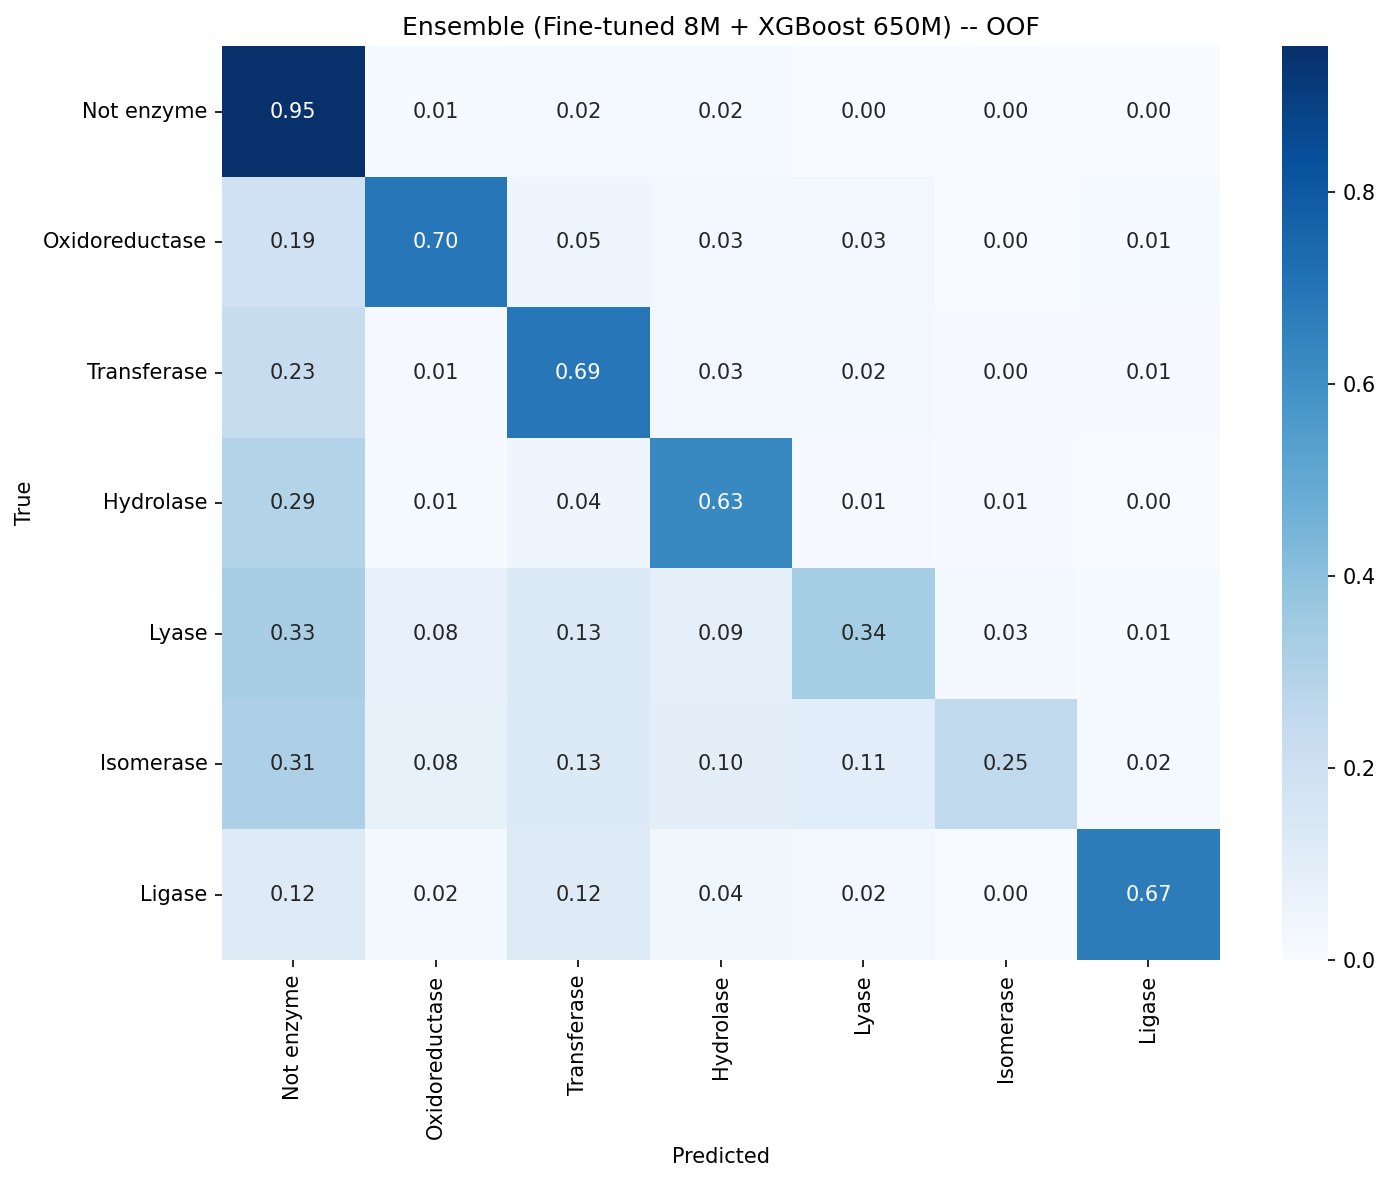
\includegraphics[width=0.85\textwidth]{../figures/cm_ensemble.png}
\caption{Ensemble confusion matrix generated from blended OOF probabilities.}
\end{figure}

\section{Extension Guide}
\subsection{Adding a New Feature Extractor}
\begin{enumerate}
\item Create \texttt{src/features/new\_feature.py} following the pattern of \texttt{composition.py}:
implement \texttt{extract\_new\_features(sequences)} $\to$ \texttt{np.ndarray} and
\texttt{get\_feature\_names()} $\to$ \texttt{list[str]}.
\item Add the new features to the ablation study in \texttt{src/models/advanced.py}.
\item Update \texttt{src/predict\_blind.py} to handle the new feature source.
\end{enumerate}

\subsection{Adding a New Model}
\begin{enumerate}
\item Create a factory function in \texttt{src/models/} (e.g.\ \texttt{make\_catboost()}).
\item Call it through \texttt{cross\_validate\_model} in \texttt{src/training.py}.
\item Add the results to the comparison table in \texttt{src/evaluation.py}.
\end{enumerate}

\subsection{Upgrading the ESM-2 Model}
To fine-tune \texttt{esm2\_t33\_650M\_UR50D} instead of the 8M model:
\begin{enumerate}
\item Update \texttt{ESM\_MODEL\_NAME} and \texttt{EMB\_DIM} in \texttt{src/models/finetune.py}.
\item Reduce \texttt{MAX\_LEN} and \texttt{batch\_size} to fit in VRAM (24 GB+ recommended).
\item Consider freezing early transformer layers to reduce memory usage.
\end{enumerate}

\subsection{Potential Improvements}
\begin{table}[H]
\centering
\caption{Candidate improvements with estimated impact and implementation difficulty.}
\begin{tabular}{lll}
\toprule
Improvement & Expected Impact & Difficulty \\
\midrule
Fine-tune 650M model & $+$5--10\% Macro F1 & High (24 GB+ VRAM) \\
Focal loss in fine-tuning & $+$2--5\% on minority classes & Medium \\
Hierarchical classification & $+$1--3\% Macro F1 & Medium \\
Per-class threshold tuning (ensemble) & $+$0.5--1\% & Low \\
Sequence-level attention visualisation & Interpretability only & High \\
\bottomrule
\end{tabular}
\end{table}

\section{Troubleshooting}
\subsection{CUDA Out of Memory}
Reduce batch size, reduce max sequence length (\texttt{--max-len 256}),
or increase gradient accumulation (\texttt{--grad-accum 8}) to maintain effective batch size.

\subsection{ESM-2 Model Download Fails}
The \texttt{fair-esm} library downloads model weights on first use.
If behind a firewall, download the checkpoint manually from the ESM GitHub repository
and place it in the \texttt{torch.hub} cache directory.

\subsection{SMOTE Failure}
SMOTE requires at least $k\_\mathrm{neighbors} + 1$ samples per class.
With default $k = 5$, classes with $\le 5$ samples will fail.
Our smallest class (Ligase, $n = 282$) is well above this threshold,
but if you subsample the data, reduce \texttt{k\_neighbors} accordingly.

\subsection{Dimension Mismatch in Blind Prediction}
When changing feature source or ESM model size, retrain and resave artifacts
so expected feature dimensionality remains consistent.

\section{Appendix: Output File Reference}
\subsection{JSON Result Files}
\begin{table}[H]
\centering
\caption{JSON result files produced by each training phase.}
\begin{tabular}{ll}
\toprule
File & Content \\
\midrule
\texttt{baseline\_results.json} & 3 baseline models: per-fold and summary metrics \\
\texttt{advanced\_results.json} & 5 advanced models + 4 ablation configs + best-model params \\
\texttt{finetune\_results.json} & 5-fold fine-tuning metrics + configuration \\
\texttt{ensemble\_results.json} & Ensemble weights, thresholds, blended metrics \\
\texttt{confidence\_results.json} & Per-level accuracy and mean probability \\
\texttt{interpretability\_results.json} & Top features, per-class metrics, high-confidence errors \\
\bottomrule
\end{tabular}
\end{table}

\subsection{Model and Cache Artifacts}
\begin{table}[H]
\centering
\caption{Model artefacts and their approximate sizes.}
\begin{tabular}{lll}
\toprule
File & Content & Size \\
\midrule
\texttt{best\_model.joblib} & XGBoost + scaler + thresholds + OOF data & $\approx$50 MB \\
\texttt{finetune\_artifact.joblib} & \texttt{FinetunePredictor} (lazy-loads PyTorch model) & $\approx$1 MB \\
\texttt{finetune\_final.pt} & PyTorch state dict (full-dataset retrained) & $\approx$35 MB \\
\texttt{finetune\_fold\{1--5\}.pt} & Per-fold best checkpoints & $\approx$35 MB each \\
\texttt{xgb\_oof\_proba.npy} & XGBoost OOF probability arrays & $\approx$2 MB \\
\texttt{xgb\_oof\_true.npy} & OOF true label array & $<$1 MB \\
\bottomrule
\end{tabular}
\end{table}

\end{document}
